\usepackage{enumitem}
\chapter{AI Component Design}
\label{ch:ai-component-design}

\section{Business Context and AI Integration}
\label{sec:business-context}

\begin{figure}[H]
    \centering
    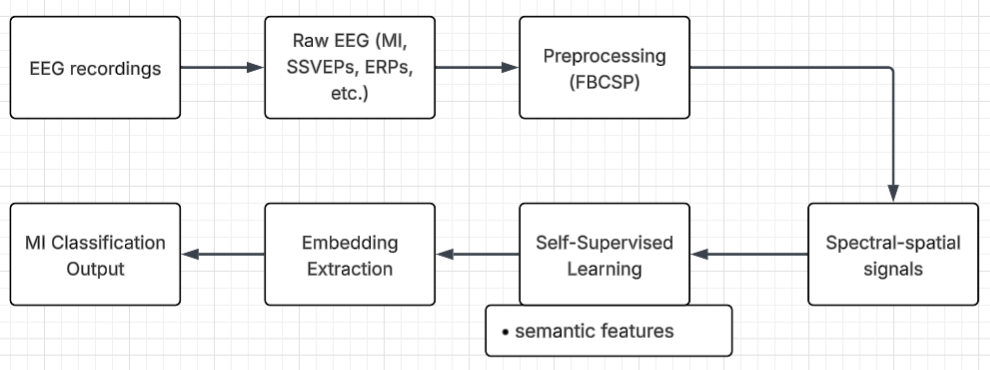
\includegraphics[width=0.95\textwidth]{figures/ssl-workflow.png}
    \caption{Proposed system workflow: Self-supervised learning for semantic feature extraction from EEG signals.}
    \label{fig:ssl-workflow}
\end{figure}

\vspace{1em}
\noindent\textbf{Why is AI suitable for this problem?}
\begin{itemize}
    \item EEG signals are complex, high-dimensional, and noisy.
    Rule-based or manually designed systems are not scalable or adaptable across paradigms.
\end{itemize}

\vspace{0.5em}
\noindent\textbf{Is the problem large, complex, or always changing?}
\begin{itemize}
    \item Yes.
    The system must generalize across multiple EEG types (MI, SSVEP, ERP) and accommodate unseen subjects and sessions.
    The input data structure and classification objectives can vary significantly.
\end{itemize}

\vspace{0.5em}
\noindent\textbf{Can we accept an answer that’s not 100\% perfect?}
\begin{itemize}
    \item Yes.
    In a research context, the goal is to improve MI classification performance over existing baselines.
    Absolute accuracy is not required — approximate, generalizable solutions are valuable.
\end{itemize}

\section{Goal Hierarchy}
\label{sec:goal-hierarchy}

\noindent\textbf{Organizational Goal:} Advance EEG-based research and improve MI classification reliability with minimal annotation cost.

\vspace{0.5em}
\noindent\textbf{System Goal:} Enable EEG researchers to conduct multi-paradigm feature learning using a unified, self-supervised architecture.

\vspace{0.5em}
\noindent\textbf{User Goal:} Simplify the research process by automating preprocessing, training, evaluation, and comparison through an integrated system.

\vspace{0.5em}
\noindent\textbf{AI Model Goal:} Learn general-purpose EEG embeddings using contrastive SSL and boost MI classification accuracy using transferred representations.

\vspace{1em}
\noindent\textbf{Success Metrics:}
\begin{itemize}
    \item Accuracy, F1-score, Precision, Recall.
    \item Robust cross-subject generalization.
    \item Automation of model training with minimal user input.
\end{itemize}

\section{Task Requirements Analysis Using AI Canvas}
\label{sec:ai-canvas}

\subsection{AI Task Requirements}
\label{subsec:ai-task-requirements}
\begin{itemize}[leftmargin=3.5em]
    \item \textbf{Requirements (REQ):} Learn semantic EEG features across MI, SSVEP, and ERP signals using unlabeled data.
    \item \textbf{Specifications (SPEC):} Investigate how SSL-based representations improve MI classification accuracy and generalization.
    \item \textbf{Environment (ENV):} Evaluated using EEG datasets like BCIC2a and OpenBMI under varying conditions (e.g., noise, subject variation).
\end{itemize}

\subsection{AI Canvas Summary}
\label{subsec:ai-canvas-summary}
\begin{itemize}[leftmargin=3.5em]
    \item \textbf{Input:} EEG signal segments from multiple paradigms (preprocessed).
    \item \textbf{Output:} Semantic embeddings and MI class predictions.
    \item \textbf{Success Criteria:} $>$80\% accuracy on unseen subjects; generalization across tasks and datasets.
\end{itemize}

\subsection{Innovation}
\label{subsec:innovation}
\begin{itemize}[leftmargin=3.5em]
    \item Unified preprocessing and SSL framework compatible with BIDS datasets.
\end{itemize}

\section{User Experience Design with AI}
\label{sec:ux-ai}

The system is fully automated and requires minimal manual intervention. Researchers interact through a web-based interface that handles dataset selection, model configuration, training, and evaluation.

\vspace{0.5em}
\noindent\textbf{UI Components:}
\begin{itemize}
    \item \textbf{Train Tab:} Select datasets, configure SSL model, and start training.
    \item \textbf{Predict Tab:} Upload EEG samples and view predicted labels with confidence scores.
    \item \textbf{Evaluate Tab:} Visualize evaluation metrics such as accuracy, F1-score, confusion matrix.
    \item \textbf{Compare Tab:} Compare SSL and supervised models across datasets and tasks.
\end{itemize}

\vspace{0.5em}
\noindent\textbf{Feedback Loop:}
Evaluation results and logs can be downloaded.
The user can reconfigure parameters and retrain models based on experiment goals.

\section{Deployment Strategy}
\label{sec:deployment}


\subsection{Deployment Plan}
\label{subsec:deployment-plan}
\begin{itemize}[leftmargin=3.5em]
    \item \textbf{Platform:} Supports local execution and GPU-enabled cloud deployment.
    \item \textbf{Architecture:} Modular backend with Flask or Streamlit; clean UI using Tailwind CSS.
    \item \textbf{Libraries:} TensorFlow/Keras, NumPy, scikit-learn, Matplotlib.
    \item \textbf{Versioning and DevOps:} Git-based version control and Docker support (planned) for reproducibility.
\end{itemize}


\subsection{Proof of Concept}
\label{subsec:proof-of-concept}
\begin{itemize}[leftmargin=3.5em]
    \item SSL-trained model (on BCIC2a): 85.4\% accuracy.
    \item Supervised EEGNet baseline: 69.5\% accuracy.
    \item Results validate the benefit of semantic feature transfer from unlabeled EEG paradigms to MI classification.
\end{itemize}

\section{Reflection and Future Development}
\label{sec:reflection}


\subsection*{Lessons Learned}
\begin{itemize}[leftmargin=3.5em]
    \item SSL can extract high-quality embeddings from unlabeled EEG data that generalize to MI classification tasks.
    \item Multi-paradigm training (e.g., SSVEP + ERP) provides richer features than MI alone.
\end{itemize}


\subsection*{Challenges}
\begin{itemize}[leftmargin=3.5em]
    \item Temporal alignment and signal variability across EEG paradigms.
    \item Visualizing and interpreting high-dimensional learned representations.
\end{itemize}

\subsection*{Future Work}
\begin{itemize}[leftmargin=3.5em]
    \item Introduce transformer-based models for long-range EEG dependencies.
    \item Deploy a live MI classification demo with real-time prediction.
\end{itemize}
